\chapter{Análise Bibliográfica sobre o Uso da Tecnologia Blockchain na Área da Saúde, por Bruno Esteves Dalla Costa Filho}

\section{Planejamento do estudo}
A blockchain é um livro-razão compartilhado e imutável que facilita o processo de registro de transações e o rastreamento de ativos em uma rede empresarial. Um ativo pode ser tangível (uma casa, um carro, dinheiro, terras) ou intangível (propriedade intelectual, patentes, direitos autorais e criação de marcas). Praticamente qualquer item de valor pode ser rastreado e negociado em uma rede de blockchain, o que reduz os riscos e os custos para todos os envolvidos.

Ela proporciona segurança de dados para armazenamento devido a criptografia e aos mineradores que verificam cada bloco, tornando a segurança um de seus principais pilares. E de fato, podemos afirmar que o uso do blockchain na saúde é bastante promissor ao garantir segurança extrema de dados, armazenar as informações médicas do paciente e ampliar o acesso ao histórico do paciente, de ensaios clínicos e resultados de novas pesquisas ainda sigilosos.

O estudo do uso da blockchain na área da saúde pode ser focado em:

\begin{itemize}
    \item Quais as possibilidades de uso dessa tecnologia fora da área de finanças?
    \item Como as características da blockchain se encaixam com as necessidades da área da saúde?
\end{itemize}

\subsection{Software de Pesquisa}

Com o uso do Bibliometrix, uma biblioteca da linguagem R amparada pelo R Studio, podemos separar e analisar informações e estatísticas sobre pesquisas científicas e seus temas.

Juntamente com a separação de dados, o Bibliometrix vem com o Biblioshiny que nos proporciona métodos para análise gráfica do estudo realizado, facilitando o entendimento pelo meio visual.

Com o uso dessas duas ferramentas permite a realização do estudo mencionado anteriormente.

\subsection{Limitações}
O estudo foi feito com poucas horas de trabalho graças as facilitações das ferramentas descritas acima.

\section{Coleta de Dados}
A coleta de dados foi feita a partir da base Web of Science no dia 3 de fevereiro de 2022, acessado pelo Portal de Periódicos da CAPES.

\section{Query de Busca}
A busca foi feita apenas com o intuito de encontrar relações entre a tecnologia Blockchain e a Área da Saúde, com um total encontrado de 1126 registros.

\begin{lstlisting}[basicstyle = \normalsize]
    ((blockchain) and (Health))
    \end{lstlisting}

\section{Análise dos dados}

\subsection{Filtragem de registros}
Antes de prosseguir com a análise, uma filtragem dos registros é feita para que se tenha como resultado somente registros de artigos publicados em revistas científicas. Dessa forma, com os 2097 registros inicias, chega-se, no final, ao número de 1834 registros.

\subsection{Análise descritiva do \textit{dataset}}

As informações sobre o \textit{dataset} a partir do Biblioshiny estão descritas a seguir:

\begin{description}
    \item [\textit{Timespan}] Entre os registros obtidos após a filtragem tem-se artigos publicados no período de 2014 a 2022
    \item [\textit{Sources (Journals, Books, etc)}] Obteve-se 584 fonte diferentes para a origem dos registros
    \item [\textit{Average years from publication}] A média do tempo de publicação dos artigos é de 2.09 anos.
    \item [\textit{Average citations per documents}] Cada artigo do \textit{dataset} foi citado em média 11.84 vezes.
    \item [\textit{Average citations per year per doc}] Após a publicação dos artigos, eles foram citados, em média, 3.319 vezes.
    \item [\textit{References}] O total de artigos obtidos possuem juntos 37816 referências citadas.
    \item [\textit{Keywords Plus (ID)}] foram obtidos 906 palavras-chave do tipo Keywords Plus (ID).
    \item [\textit{Author's Keywords (DE)}] 2514 palavras-chave indicadas pelos autores foram encontradas nos registros  .
    \item [\textit{Authors}] 3875 nomes de autores foram encontrados no \textit{dataset}  
    \item [\textit{Author Appearances}] Os 3875 distintos autores foram encontrados 4744 vezes, como autores de artigos.
    \item [\textit{Authors of single-authored documents}] Dentre os 3875 autores encontrados, 60 deles editaram artigos individualmente.
    \item [\textit{Authors of multi-authored documents}] Dentre os 3875 autores encontrados, 3815 deles editaram artigos com um ou mais co-autores.
    \item [\textit{Single-authored documents}] Dentre os artigos encontrados no \textit{dataset}, 62 foram escritos por um único autor.
    \item [\textit{Documents per Author}] Entre os 3875 autores, cada um publicou em média 0.291 documentos.
    \item [\textit{Authors per Document}] Cada um dos artigos encontrados no \textit{dataset} foi autorado, em média, com 3.44 autores.
    \item [\textit{Co-Authors per Documents}] As 4744 aparições autores se distribuem, em média 4.21 vezes para os documentos.
    \item [\textit{Collaboration Index}] Os 3875 nomes de autores que editaram artigos com um ou mais co-autores, colaboraram em media 3.59 vezes.
\end{description}

\subsection{Evolução da produção científica}

Usando o Bibliometrix pode-se obter um gráfico que mostra a produção científica anual sobre o tema em questão. O gráfico obtido é o seguinte:


\begin{figure}[H]
    \centering
    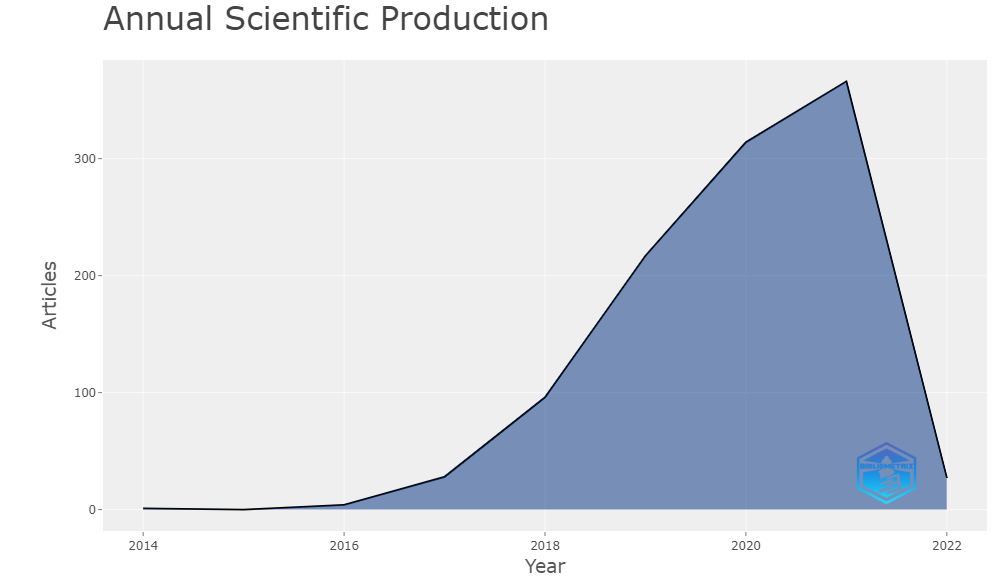
\includegraphics[width=1\textwidth]{experiments/brunoedcf/AnaliseBibliometrica/BlockchainInHealth/Figures/AnualCientProd.png}
    \caption{Evolução da produção científica no \dataset}
\end{figure}